\documentclass[conference]{IEEEtran}
\IEEEoverridecommandlockouts
\usepackage[utf8]{inputenc}
\usepackage{cite}
\usepackage{amsmath,amssymb,amsfonts}
\usepackage{algorithmic}
\usepackage{graphicx}
\usepackage{textcomp}
\usepackage{xcolor}
\usepackage{booktabs}
\usepackage{colortbl}
\usepackage{multirow}
\usepackage{tikz}
\usetikzlibrary{arrows.meta, positioning, fit}
\def\BibTeX{{\rm B\kern-.05em{\sc i\kern-.025em b}\kern-.08em
    T\kern-.1667em\lower.7ex\hbox{E}\kern-.125emX}}
\begin{document}

\title{RGB-Only Driver State Monitoring for Embedded Deployment: A Model Comparison Study\\
\thanks{}
}

\author{\IEEEauthorblockN{Khongmeng Kormoua}
\IEEEauthorblockA{\textit{Electrical and Computer Engineering} \\
\textit{University of St. Thomas}\\
Saint Paul, United States \\
korm4202@stthomas.edu}
\and
\IEEEauthorblockN{Cheol-Hong Min}
\IEEEauthorblockA{\textit{Electrical and Computer Engineering} \\
\textit{University of St. Thomas}\\
Saint Paul, United States \\
cmin@stthomas.edu}
}

\maketitle

\begin{abstract}
% TODO(author): trim/adjust once happy with the numbers.
Distracted and drowsy driving are still one of the biggest causes of crashes on the road today. A driver monitoring system (DMS) that can watch the driver continuously and warn them before something bad happens could help a lot with this problem. Many DMS designs on the market or in research use infrared cameras, depth sensors, or wearable biosensors to make the system more reliable in bad lighting, but all of these add cost and make the system harder to install in a normal vehicle. This paper looks at the opposite direction: build a driver state monitoring pipeline using only one regular RGB camera, and design it so it can eventually run on a small embedded computer, the NVIDIA Jetson Orin Nano Super. The pipeline uses a chain of pretrained models to get face location, head pose, eye state, gaze direction, and mouth shape from each frame, turns these into a 13-number feature vector, and then a temporal model decides the driver's state from the sequence of these numbers. Since we did not fine-tune any of the upstream models, the only thing we actually train is this last classifier, so the paper focuses on comparing ten different architectures for it, from classic machine learning (SVM, Random Forest, Gradient Boosted Trees) to recurrent and convolutional sequence models (GRU, Temporal Convolutional Network) to models trained directly on raw pixels (a fine-tuned ResNet18+GRU and a 3D-CNN). All ten are trained and tested on the same driver-independent split of the Driver Monitoring Dataset (DMD), so the comparison is fair. The best result comes from averaging two GRU models together (a gated dual-branch GRU and a plain single-branch GRU), giving a macro-F1 of 0.810 using only 84,609 parameters combined, which is much smaller than the raw-pixel models we also tested (up to 33.2 million parameters) even though it performs better. We also found that using raw pixels does not actually beat the best hand-engineered-feature models here, and that training one of the models longer actually made it slightly worse. We further port the full pipeline to the Jetson Orin Nano Super and measure it directly: as TensorRT FP16 engines the cascade plus classifier runs in about 5\,ms per frame (roughly 200\,fps of compute) while drawing under 10\,W and using 4.1\,GB of memory, confirming that the design fits the embedded budget with large margin.
\end{abstract}

\begin{IEEEkeywords}
driver monitoring system, driver state classification, embedded deep learning, gated recurrent unit, temporal convolutional network, DMD dataset
\end{IEEEkeywords}

\section{Introduction}

Distracted driving and drowsy driving are two of the leading causes of crashes on the road \cite{b_cdc}, and both are things that a good driver monitoring system could catch before an accident happens. There are already many ways researchers have tried to solve this problem. Some approaches put sensors directly on the driver, such as an EEG headset that reads brain activity to estimate how attentive the driver currently is \cite{b_wearable}. This kind of wearable approach can work well, but it requires the driver to wear something, which is not always practical for a system that is supposed to run every time someone drives. Camera-based systems avoid this problem completely, since the driver does not have to wear or touch anything, the camera just watches them.

However, most camera-based driver monitoring papers we found do not use a plain RGB camera by itself. Many of them add an infrared camera and IR illuminator so the system still works at night or in bad lighting \cite{b_riskaware}, or they combine the camera with physiological sensors such as heart rate or skin conductance to make the prediction more reliable \cite{b_riskaware}. These are reasonable choices, but they also mean more hardware, more wiring, and more cost, which matters a lot if the goal is eventually to put this system in an ordinary car rather than a research vehicle.

This paper looks at the case where none of that extra hardware is available, only a single RGB camera and a small embedded computer, specifically the NVIDIA Jetson Orin Nano Super. Under this constraint, the question we care about is not just how accurate can the system be, but which architecture actually makes sense once we also have to worry about how much compute it needs, since an embedded board cannot just run the biggest and most accurate model available.

The Driver Monitoring Dataset (DMD) \cite{b_dmd} is, as far as we know, the largest public dataset that has both drowsiness and distraction annotations recorded from real drivers, and it is the dataset used for all of the results in this paper. The DMD paper itself does not report any classification results, it is a dataset paper. The only other classification result on DMD that we found used only 5 subjects and a subject-dependent split \cite{b_dmd_canas}, meaning the same driver could appear in both the training and test data, which makes it hard to compare directly to what we report here, since our split never lets a driver appear in both. A closer point of comparison is the UTA-RLDD dataset \cite{b_utarldd}, which is also subject-independent and also splits driver state into three stages; the baseline model published with that dataset reports 65.2\% accuracy.

Two recent papers are close to what we are trying to do here. Scribano et al. \cite{b_scribano} built a small multi-task network that predicts landmarks, eye state, mouth state, head pose, and a distraction label all from one frame, and tested it on a Jetson Nano and a Jetson Xavier NX, getting under 2\,ms per frame for their smallest model. The problem is that their network has no memory between frames at all, every prediction only looks at the current image, so there is no way for it to compute something like PERCLOS, which needs to look at eye closure over a window of time, not just one instant. Another paper, targeting the Jetson Orin Nano directly \cite{b_multiregion}, uses a shared MobileNetV3-Small backbone over several image regions and smooths the output with an exponential moving average. This is closer to temporal reasoning, but an EMA is still just a fixed decay filter on the output, not something that learned how to integrate information over time, and neither of these papers actually tries to separate drowsiness from general fatigue, which is exactly the kind of thing that needs real temporal modeling to work at all.

There is also a question of whether raw video is even a good input in the first place, compared to hand-picked features like head pose and eye state. Ma et al. \cite{b_ma2022} found that a 2D-CNN working frame by frame matched or beat a 3D-CNN video model for driver monitoring at a similar number of subjects to what we have here, while also being much faster. Li et al. \cite{b_imagepretrain} found something similar in a more general video setting: image-pretrained 2D models transfer better than video-pretrained 3D models specifically when there is not much video data to fine-tune on. Both of these match what we found in our own experiments, described in Section~\ref{sec:results}: with only 14 drivers total, giving the model more spatiotemporal capacity to work with does not actually help.

The rest of this paper is organized as follows. Section~\ref{sec:design} describes the dataset, the feature-extraction pipeline, and the ten classifier architectures we compared. Section~\ref{sec:results} reports the comparison and discusses what we found, including two results we did not expect going in. Section~\ref{sec:embedded} discusses what this means for running the system on the Jetson, and Section~\ref{sec:conclusion} concludes and lists what is left to do.

\section{System Design}
\label{sec:design}

\begin{figure}[htbp]
  \centering
  \begin{tikzpicture}[
      node distance=6pt and 10pt,
      block/.style={draw, rounded corners, minimum height=0.7cm, minimum width=2.6cm, align=center, font=\scriptsize, fill=blue!6},
      small/.style={draw, rounded corners, minimum height=0.6cm, minimum width=2.2cm, align=center, font=\scriptsize, fill=gray!8},
      arr/.style={-Stealth, thick}
    ]
    \node[block] (face) {① SCRFD-500M\\face detect};
    \node[small, below=of face] (pose) {② 6DRepNet\\head pose};
    \node[small, below=of pose] (eye) {③ eye-state\\open/closed};
    \node[small, below=of eye] (gaze) {⑤ gaze\\yaw/pitch};
    \node[small, below=of gaze] (mouth) {2d106det\\MAR / yawn};
    \node[block, right=16pt of eye] (temporal) {Temporal:\\PERCLOS, blink\\rate, yawn rate};
    \node[block, right=16pt of temporal] (clf) {Stage-4\\Classifier\\(10 compared)};
    \node[small, right=16pt of clf] (state) {FOCUSED /\\DISTRACTED /\\FATIGUED /\\NO\_FACE};

    \draw[arr] (face) -- (pose);
    \draw[arr] (face) -- (eye);
    \draw[arr] (face) -- (gaze);
    \draw[arr] (face) -- (mouth);
    \draw[arr] (pose.east) -- ++(0.3,0) |- (temporal.west);
    \draw[arr] (eye.east) -- (temporal.west);
    \draw[arr] (gaze.east) -- ++(0.3,0) |- (temporal.west);
    \draw[arr] (mouth.east) -- ++(0.3,0) |- (temporal.west);
    \draw[arr] (temporal) -- (clf);
    \draw[arr] (clf) -- (state);
  \end{tikzpicture}
  \caption{Overall pipeline. Everything before the classifier box is a pretrained model that we did not train ourselves, only the last classifier stage is trained.}
  \label{fig:pipeline}
\end{figure}

\subsection{Dataset}

We used the Driver Monitoring Dataset (DMD) \cite{b_dmd}, which has two protocols that matter for this work: a drowsiness protocol, with eye state, blink, and yawn labels, and a distraction protocol, with gaze-on-road and driver-action labels. We used 65 sessions covering 14 different drivers total. After extracting features every second frame (about 15\,fps effective) and dropping frames where no face was detected, the final labeled table has 214,680 frames.

\subsection{Feature-Extraction Cascade}

Fig.~\ref{fig:pipeline} shows the full pipeline. Every stage before the final classifier is a model we did not train, we just used the pretrained weights as they are, since composing existing models is much more realistic than training a large model from scratch on only 14 drivers' worth of data. The stages are:
\begin{itemize}
    \item[①] Face detection with SCRFD-500M \cite{b_scrfd}, which gives a bounding box and 5 keypoints.
    \item[②] Head pose with 6DRepNet \cite{b_6drepnet}, giving yaw, pitch, and roll.
    \item[③] Eye state with open-closed-eye-0001 \cite{b_openvino_eye}, a small model that tells if each eye is open or closed.
    \item[⑤] Gaze with gaze-estimation-adas-0002 \cite{b_openvino_gaze}, which takes the eye crops and head pose and gives gaze yaw/pitch.
    \item Mouth and yawn: there is no pretrained mouth-open/closed model like there is for eyes, so we instead use 106-point facial landmarks (2d106det) to compute a Mouth Aspect Ratio (MAR) ourselves.
\end{itemize}
After these per-frame signals are computed, a temporal layer turns them into rolling statistics, the most important one being PERCLOS (the fraction of time the eyes were closed over a window), along with blink rate and yawn rate. We also compute short 5-second rolling statistics of head pose and gaze, so the model can tell a sustained head turn apart from a quick glance. In total, 13 numbers are passed to the classifier for every frame: yaw, pitch, eye-open probability, PERCLOS, blink rate, gaze yaw, gaze pitch, a 15-second PERCLOS variant, 5-second rolling standard deviation of yaw and gaze yaw, 5-second rolling mean of eye-open probability, MAR, and yawn rate.

\subsection{Label Taxonomy}
\label{sec:taxonomy}

We originally wanted 4 driver states (FOCUSED, DISTRACTED, DROWSY, TIRED) plus a NO\_FACE fallback for frames where the driver is not detected. In practice, DROWSY and TIRED each only make up about 2.7--2.8\% of the labeled frames, since only 14 drivers were available, which is not enough data to learn these as two separate classes without the model just overfitting to a handful of drivers. Fig.~\ref{fig:classdist} shows this directly: DISTRACTED and FOCUSED together make up about 94\% of the data, leaving DROWSY and TIRED at only 5.6\% combined. Because of this, we merged DROWSY and TIRED into one FATIGUED class for every classifier trained in this paper, giving 3 states total (FOCUSED, DISTRACTED, FATIGUED) plus NO\_FACE. This was not really a design choice we wanted to make, it came directly from testing the 3-class and 4-class versions and seeing that 4-class simply did not have enough data per class to work. Splitting FATIGUED back into DROWSY and TIRED is something we would like to revisit if more drivers become available later. This same imbalance is also the reason we use macro-F1 instead of plain accuracy for every result in this paper (Section~\ref{sec:results}).

\begin{figure}[htbp]
  \centering
  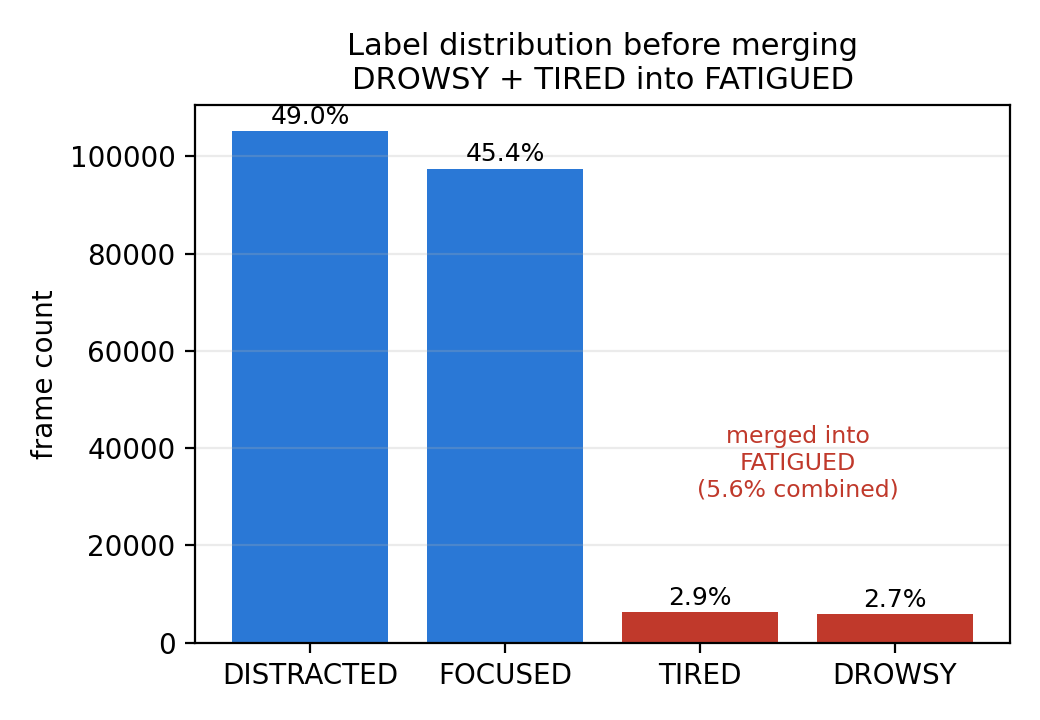
\includegraphics[width=0.42\textwidth]{figure/class_distribution.png}
  \caption{Frame counts for the original 4-state labels before merging. DROWSY and TIRED are each under 3\% of the data on their own.}
  \label{fig:classdist}
\end{figure}

\subsection{Classifier Architectures}
\label{sec:classifiers}

All ten architectures below were trained and evaluated on the same driver-independent split, 10 drivers for training and 4 drivers held out completely for evaluation, meaning the held-out drivers were never used for training or even for picking the best checkpoint. Every architecture that trains iteratively was trained for a full 200 epochs, so the comparison stays fair across models, except for the three classical machine learning baselines, which do not train over epochs in the same sense.

The classical machine learning group (SVM with an RBF kernel, Random Forest, and Gradient Boosted Trees) all take the 13-number feature vector for a single frame, with no memory of previous frames at all. The MLP is a small per-frame neural network on the same 13 numbers, also with no temporal memory.

For sequence models on top of the hand-engineered features, we tried a Temporal Convolutional Network (TCN) \cite{b_tcn}, a single-branch Gated Recurrent Unit (GRU) \cite{b_gru}, and what we call a Gated-Fatigue GRU. This last one is a dual-branch design: one GRU branch sees all 13 features and predicts FOCUSED/DISTRACTED, while a second, completely separate GRU branch only sees the eye/PERCLOS/yawn-related features and predicts FATIGUED. The idea is that head pose and gaze should have no way to influence the fatigue decision at all, which matches how FATIGUED is actually defined in the ground truth, using only eye closure and yawning, never head pose.

Finally, we tried two models that work directly on raw pixels instead of the 13 hand-engineered features, to see whether a learned representation could do better: a ResNet18 backbone (with the last residual block fine-tuned) feeding into a GRU, and R3D-18, a 3D-CNN clip classifier pretrained on Kinetics-400.

\subsection{Ensembling}

The best result we got was simply averaging the softmax probabilities of the single-branch GRU and the Gated-Fatigue GRU together every frame, with no extra training needed. This works because the two models tend to make different kinds of mistakes on the rare FATIGUED class, the gated model is precise but a bit conservative, while the single-branch model catches more of the true FATIGUED frames but with more false positives, so averaging the two ends up better than either one alone.

\section{Results}
\label{sec:results}

\begin{figure}[htbp]
  \centering
  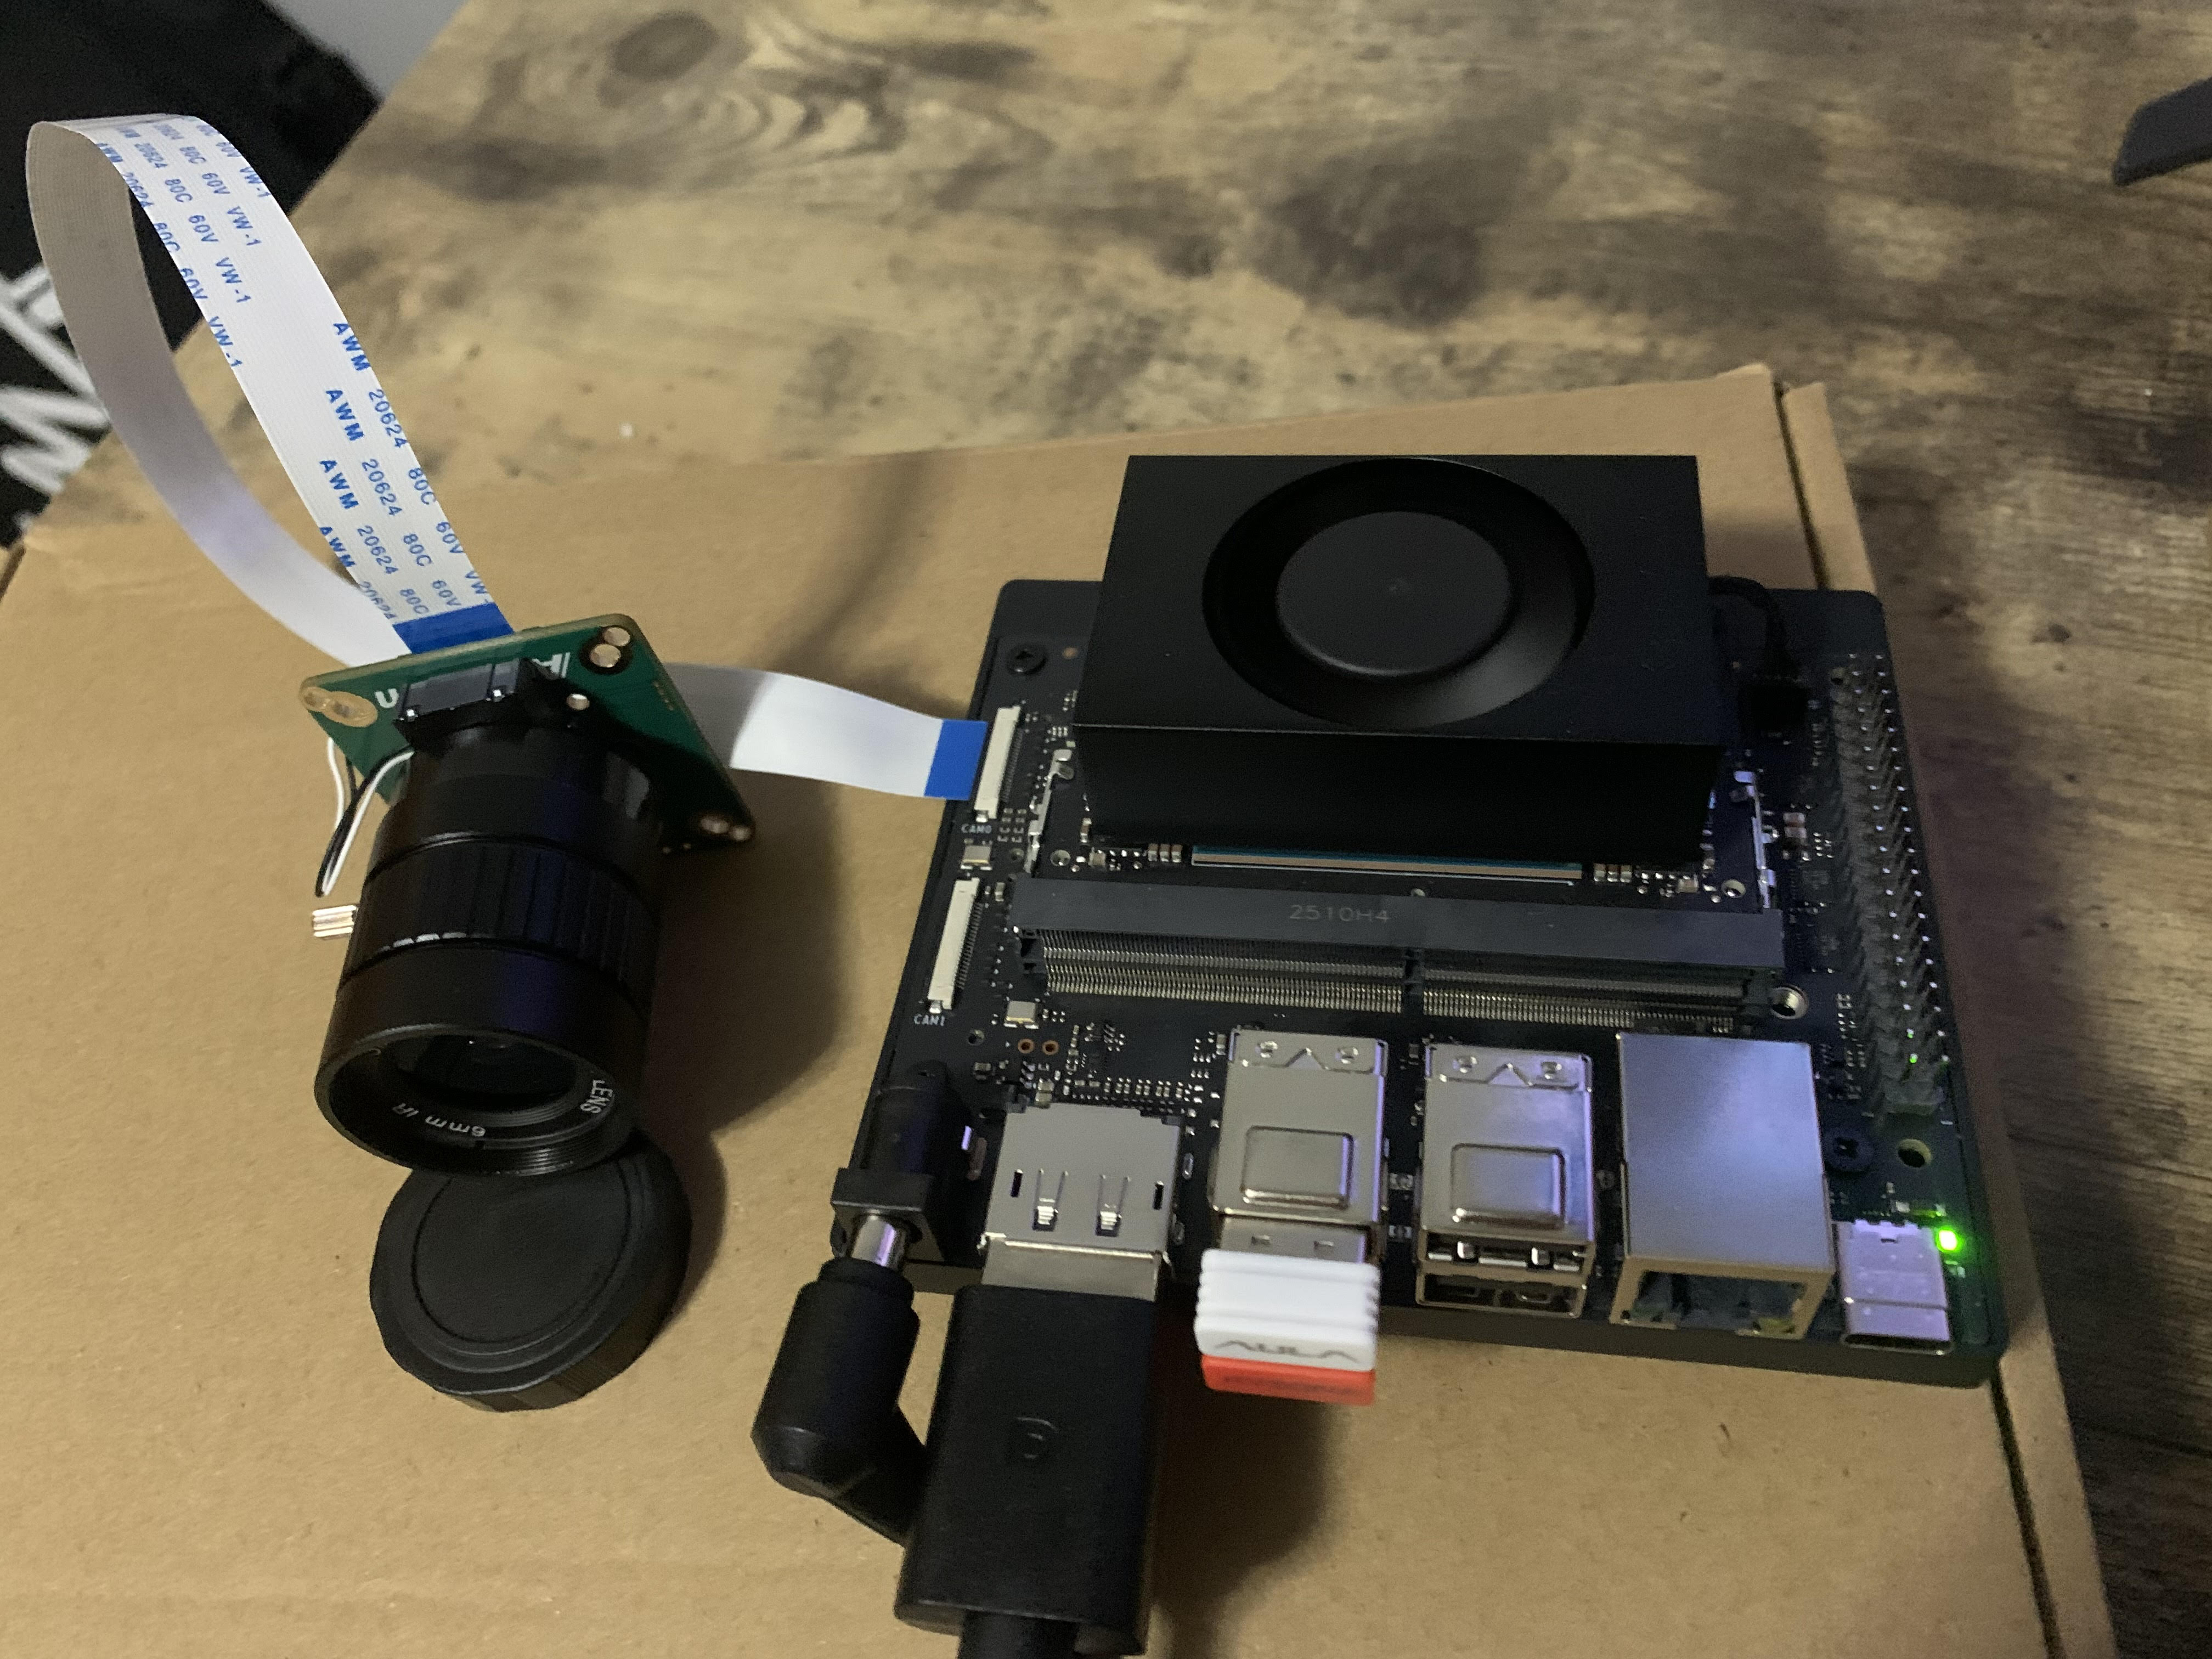
\includegraphics[width=0.48\textwidth]{figure/hardware_setup.jpg}
  \caption{The camera and Jetson used for this project: a driver-facing ArduCam IMX477 paired with the target Jetson Orin Nano Super board.}
  \label{fig:hardware}
\end{figure}

Training was done on an NVIDIA RTX 4070 Ti Super (16\,GB), and the target hardware for deployment is an NVIDIA Jetson Orin Nano Super (Fig.~\ref{fig:hardware}), which supports up to 67 INT8 TOPS and has four selectable power modes, 7\,W, 15\,W, 25\,W, and an uncapped MAXN mode \cite{b_jetson}. The camera is an ArduCam IMX477, 1280$\times$720 at 30\,fps.

For training, we used class-weighted or focal loss to deal with the class imbalance, since FATIGUED is only around 3\% of all frames. Sequence models were trained on fixed-length overlapping chunks of 600 frames (about 40 seconds, with 50\% overlap between chunks), but evaluation was done as one continuous forward pass over the full held-out session, which matches how the model would actually be used live rather than in fixed windows. We also used chunk-level oversampling instead of row-level oversampling for the sequence models, since shuffling individual rows would break the temporal order the model depends on.

We report macro-F1 as the main metric instead of plain accuracy, because FATIGUED is a small minority class and accuracy alone can look good just by mostly ignoring it. Macro-F1 weights every class equally, so it is a better way to check whether the rare but important FATIGUED class is actually being detected.

Table~\ref{tab:comparison} shows all ten architectures side by side. The best single model is the Gated-Fatigue GRU at 0.798 macro-F1, and averaging it with the single-branch GRU pushes this up to 0.810, which is the best result in this paper. Fig.~\ref{fig:ensemble_curve} shows the validation curve during training for both GRU models, along with where the final ensemble result lands. Fig.~\ref{fig:accparams} plots macro-F1 against the number of classifier parameters for every neural architecture, which is really the main point of this paper, since it shows that the best-performing models here also happen to be by far the smallest ones.

\begin{table}[htbp]
\centering
\caption{All ten architectures on the held-out driver split. Params is the trained classifier only, it does not include the pretrained cascade stages before it. The three classical ML models do not have a comparable parameter count, so they are marked N/A. Lat.\ is the measured per-frame stage-4 classifier latency on the Jetson Orin Nano Super at MAXN, and excludes the shared cascade front-end (that is reported separately in Section~\ref{sec:embedded}). Neural models are timed in PyTorch (CUDA), their present runtime; classical models ($\ddagger$) run in scikit-learn on the CPU, timed on representative inputs (their fitted models are not checkpointed), so the Random Forest figure in particular is indicative. $\dagger$: the tiny feature heads sit on a fixed ${\sim}0.5$\,ms PyTorch kernel-launch overhead, so their true compute is far smaller (0.02\,ms for the GRU under TensorRT) and parameter count is the fairer compute proxy for them. $\S$: R3D-18 emits one prediction per 16-frame clip (293\,ms/clip), so its figure is per-frame amortized.}
\label{tab:comparison}
\begin{tabular}{@{}lcccc@{}}
\toprule
\textbf{Architecture} & \textbf{Input} & \textbf{macro-F1} & \textbf{Params} & \textbf{Lat.\ (ms)} \\
\midrule
SVM (RBF) & features & 0.531 & N/A & 0.70$^\ddagger$ \\
Random Forest & features & 0.599 & N/A & 88$^\ddagger$ \\
Gradient Boosted Trees & features & 0.620 & N/A & 1.84$^\ddagger$ \\
MLP (per-frame) & features & 0.599 & 3{,}101 & 0.51$^\dagger$ \\
TCN & features, seq. & 0.720 & 139{,}549 & 4.59 \\
R3D-18 (3D-CNN) & raw pixels & 0.712 & 33{,}177{,}437 & 18.4$^\S$ \\
ResNet18+GRU (fine-tuned) & raw pixels & 0.742 & 11{,}314{,}205 & 8.54 \\
GRU (single-branch) & features, seq. & 0.790 & 40{,}349 & 0.60$^\dagger$ \\
Gated-Fatigue GRU & features, seq. & 0.798 & 44{,}260 & 1.17 \\
\textbf{Ensemble (both GRUs)} & features, seq. & \textbf{0.810} & \textbf{84{,}609} & \textbf{1.77} \\
\bottomrule
\end{tabular}
\end{table}

\begin{figure}[htbp]
  \centering
  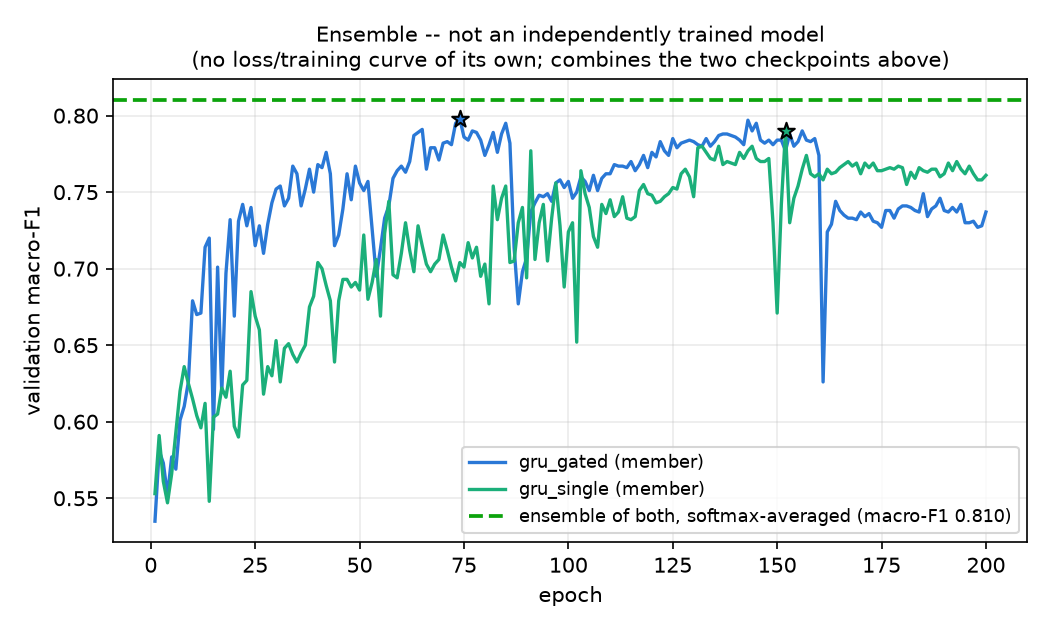
\includegraphics[width=0.48\textwidth]{figure/ensemble_curve.png}
  \caption{Validation macro-F1 during training for both GRU models, with each one's best checkpoint marked and the final ensemble score shown as a line. The ensemble itself does not have its own training curve since it is just the two checkpoints combined.}
  \label{fig:ensemble_curve}
\end{figure}

\begin{figure}[htbp]
  \centering
  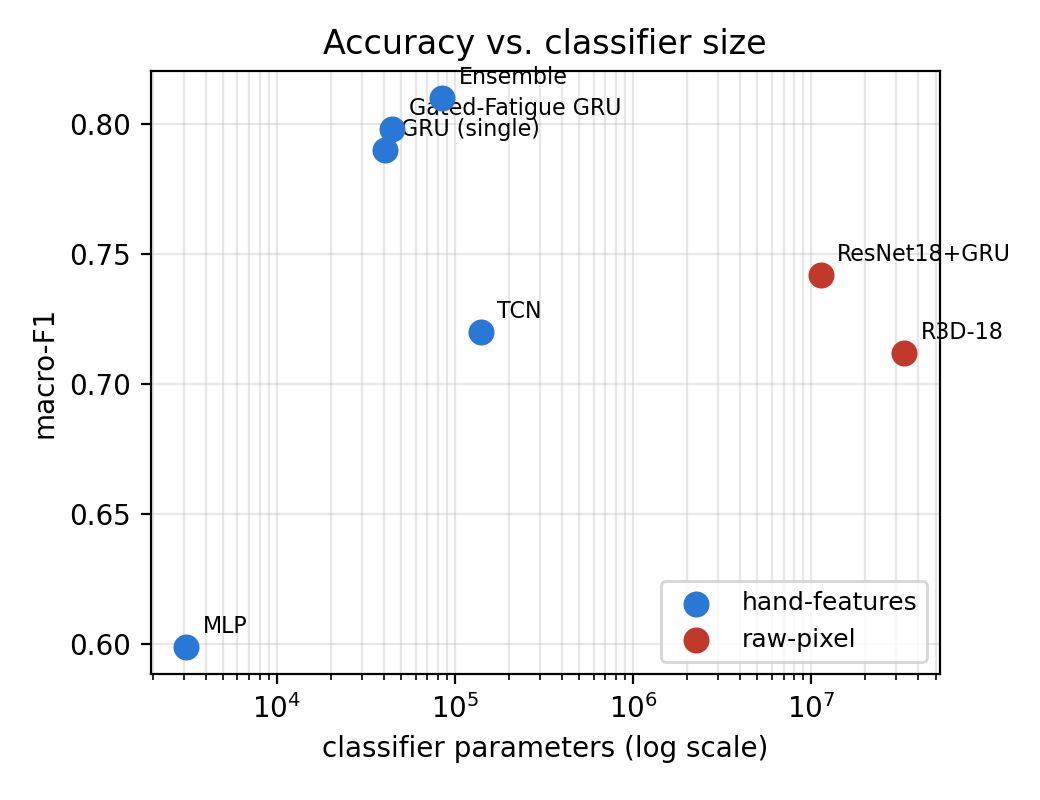
\includegraphics[width=0.48\textwidth]{figure/accuracy_vs_params.png}
  \caption{macro-F1 against classifier parameter count (log scale) for every trained neural architecture. The hand-engineered-feature GRU family sits in the top left, meaning best accuracy with the fewest parameters, while the raw-pixel models sit lower and much further right.}
  \label{fig:accparams}
\end{figure}

Looking at the final ensemble by class: FOCUSED gets 0.828 precision, 0.827 recall, 0.827 F1; DISTRACTED gets 0.881/0.864/0.872; FATIGUED gets 0.656/0.821/0.729 (support 20{,}402/25{,}666/2{,}096 frames, overall accuracy 0.846). Fig.~\ref{fig:confmat} shows the full confusion matrix. FATIGUED, which is both the rarest class and the one we care most about catching, ends up with the lowest precision of the three but the highest recall, meaning the ensemble tends to flag fatigue a bit too often rather than missing it, which is probably the right side to be wrong on for a safety warning.

\begin{figure}[htbp]
  \centering
  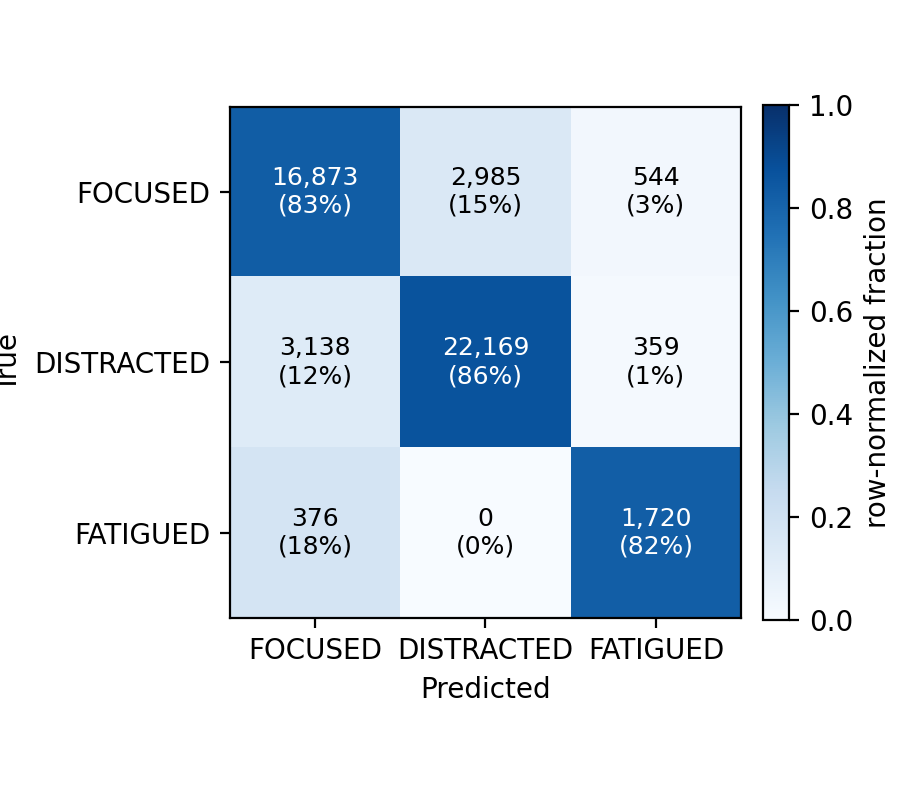
\includegraphics[width=0.42\textwidth]{figure/confusion_matrix.png}
  \caption{Confusion matrix for the final ensemble on the held-out drivers, raw per-frame (not smoothed). Numbers are frame counts with the row-normalized percentage in parentheses.}
  \label{fig:confmat}
\end{figure}

\subsection{Raw pixels do not beat the best hand-feature models here}

Both raw-pixel models come in below the GRU family (0.790--0.810), even though the fine-tuned ResNet18+GRU has over 250 times as many parameters as the Gated-Fatigue GRU. That said, it is not true that raw pixels lose across the board: the fine-tuned ResNet18+GRU (0.742) beats every classical ML baseline and the MLP by a wide margin, and it even slightly beats the hand-feature TCN (0.720). So the actual finding is narrower than ``raw pixels are worse,'' it is that raw pixels specifically do not beat the strongest recurrent hand-feature models, which is still a meaningful gap. We think the most likely explanation is the number of drivers, not the models themselves. With only 14 drivers, a large CNN has plenty of room to just memorize what each individual driver looks like (skin tone, face shape, how the light hits them) rather than learning something that generalizes to the 4 drivers it never saw during training. This lines up with what Li et al. \cite{b_imagepretrain} and Ma et al. \cite{b_ma2022} found in other video tasks with limited data. As far as we know, nobody has directly compared raw pixels against hand-engineered features under the exact same protocol for this task before, so this comparison is new even if the conclusion is not entirely surprising.

\subsection{Training longer did not help every model}

Since we wanted a fair comparison, we trained every iterative architecture for a full 200 epochs, even ones that were originally trained for far fewer. This mostly worked out fine, three out of four raw-pixel/TCN models were either unchanged or slightly better at 200 epochs. The fine-tuned ResNet18+GRU, however, actually went down, from 0.753 at its original 15-epoch budget to 0.742 once trained to 200 epochs. This is also the largest classifier in the whole comparison by parameter count (11.3 million), trained on the smallest number of training chunks of any architecture here, so it makes sense that it would be the one most likely to overfit with extra training time. We kept the 200-epoch number in Table~\ref{tab:comparison} anyway, since using the better 15-epoch number just for this one model would break the fairness of the comparison, but it is worth pointing out that more training epochs is not automatically better, at least not for the highest-capacity model in a dataset this small.

\section{Toward Embedded Deployment}
\label{sec:embedded}

Part of the reason we compared 10 different architectures instead of just picking the most accurate one is that an embedded board cannot simply run whatever gets the best number, it has to also fit inside a real-time latency and power budget. Table~\ref{tab:comparison} already tells us something useful here even without touching the Jetson: the classifier itself is a tiny part of the total compute, no matter which one we pick. Even the biggest raw-pixel model (33.2 million parameters) is small by the standards of embedded vision models, and the ensemble we are actually recommending (84,609 parameters combined) is far smaller still. The part of the pipeline that will actually decide whether this runs in real time is the cascade in Fig.~\ref{fig:pipeline}, stages ① through ⑤, since those run on every single frame no matter which classifier is used afterward.

Two papers we cited earlier already give us a rough idea of what to expect. Scribano et al. \cite{b_scribano} report 1.73\,ms per frame (FP16) for their smallest model on a Jetson Xavier NX, and 16.5--23.7\,ms for their full pipeline depending on how often face detection runs. A separate paper targeting the Jetson Orin Nano directly \cite{b_multiregion} projects 13--20\,fps for a similar single-frame network. These numbers are useful as a rough reference, but they are for different network architectures running on different (and in one case weaker) hardware than what we are using, so they cannot really substitute for actually measuring our own pipeline.

We have now ported the full pipeline to the Jetson Orin Nano Super and measured it directly. Each of the five cascade stages, and the classifier, was built as a TensorRT FP16 engine and benchmarked at the uncapped MAXN power mode; Table~\ref{tab:embedded} reports the per-stage latency. In isolation the whole cascade plus classifier sums to about 5.0\,ms per frame, roughly 200\,frames per second of compute, and is dominated by the two backbone stages, SCRFD and 6DRepNet. The classifier itself is negligible, confirming on the actual hardware what the parameter counts already suggested.

We also measured the pipeline end-to-end over a held-out DMD session (1280$\times$720, 2000 frames, all with a detected face). Our current reference implementation runs the cascade through ONNX Runtime's CUDA provider, with the gaze model on the CPU, rather than through the TensorRT engines, and sustains 11.5\,fps of compute (9.9\,fps including video decode). The gap between this and the ${\sim}200$\,fps compute bound is almost entirely because the two heaviest stages are not yet wired to their TensorRT engines: run through ONNX Runtime, 6DRepNet and SCRFD take 47.6\,ms and 22.9\,ms per frame, about 20$\times$ their standalone FP16 engine latency. Closing that gap is an implementation task, not a change to any model. Table~\ref{tab:embedded_sys} lists the system-level measurements. At MAXN the board draws only 9.5\,W on average (10.4\,W peak) and the pipeline peaks at 4.1\,GB of the 8\,GB shared memory pool, both well within budget. Since an in-vehicle system runs on vehicle power, the more relevant constraints are latency and memory, and the design meets both with large margin.

Two caveats apply. The per-stage figures in Table~\ref{tab:embedded} are standalone engine latencies and do not include the pre- and post-processing between stages (face cropping, resizing, and the detector's anchor decoding and non-max suppression), so a fully optimized end-to-end rate would fall between our measured 11.5\,fps and the 200\,fps compute bound rather than at the bound. And the stage-4 classifiers in Table~\ref{tab:comparison} are timed in PyTorch, their present runtime: the very small feature-based heads sit on a fixed PyTorch kernel-launch overhead of about half a millisecond, so their true compute (0.02\,ms for the GRU under TensorRT) is well below what that column shows, which is why parameter count remains the fairer compute proxy for them.

Fig.~\ref{fig:acclat} places all ten architectures on the axis that matters most for deployment, macro-F1 against measured per-frame latency, which is the on-device analog of the accuracy-versus-parameters view in Fig.~\ref{fig:accparams}. The hand-engineered-feature GRU family sits in the top-left corner, the best accuracy at the lowest latency, while both raw-pixel models sit lower and well to the right, and the classical baselines lower still. The model we recommend is thus not only the most accurate but also among the cheapest to run on the target board.

\begin{figure}[htbp]
  \centering
  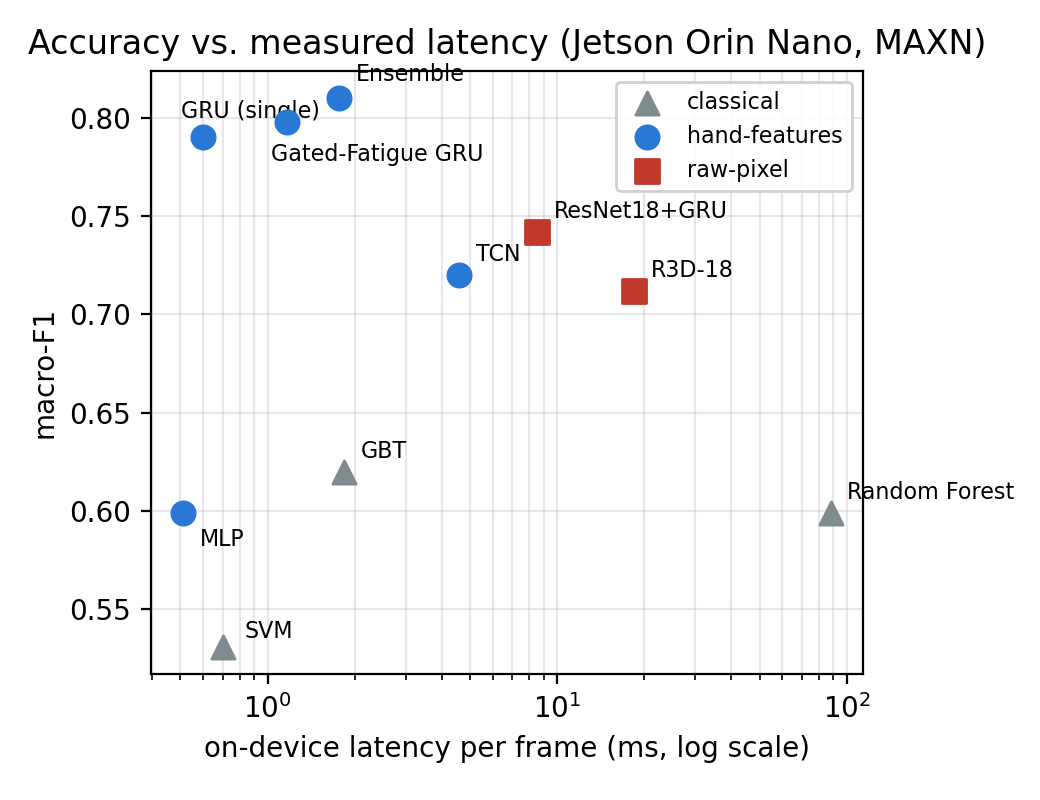
\includegraphics[width=0.48\textwidth]{figure/accuracy_vs_latency.png}
  \caption{macro-F1 against measured per-frame on-device latency (log scale) on the Jetson Orin Nano Super at MAXN, for all ten architectures. Latency is the stage-4 classifier only (neural models timed in PyTorch/CUDA, classical in scikit-learn on CPU); the shared cascade front-end is reported separately in Table~\ref{tab:embedded}. The hand-feature GRU family (top-left) reaches the highest accuracy at the lowest latency.}
  \label{fig:acclat}
\end{figure}

\begin{table}[htbp]
\centering
\caption{Measured per-stage latency on the Jetson Orin Nano Super (MAXN, TensorRT FP16, median GPU compute time). Every stage runs once per frame, except eye state, which runs once per eye. The gaze model, distributed only as OpenVINO IR, was converted to ONNX for this measurement and verified against the original to within $1.6\times10^{-3}$ on the output vector.}
\label{tab:embedded}
\begin{tabular}{@{}clc@{}}
\toprule
\textbf{Stage} & \textbf{Model} & \textbf{TRT FP16 (ms)} \\
\midrule
1 & SCRFD-500M (face detect) & 1.73 \\
2 & 6DRepNet (head pose) & 2.23 \\
3 & open-closed-eye-0001 ($\times$2) & 0.04 \\
5 & gaze-estimation-adas-0002 & 0.40 \\
-- & 2d106det (mouth / yawn) & 0.52 \\
4 & GRU ensemble (classifier) & 0.02 \\
\midrule
\multicolumn{2}{@{}l}{\textbf{Total per frame}} & \textbf{$\approx$5.0} \\
\bottomrule
\end{tabular}
\end{table}

\begin{table}[htbp]
\centering
\caption{Measured system-level performance on the Jetson Orin Nano Super at MAXN, over a held-out DMD session. The reference implementation runs the cascade in ONNX Runtime (CUDA) with the gaze model on the CPU; the compute bound is the sum of the TensorRT FP16 engines in Table~\ref{tab:embedded}.}
\label{tab:embedded_sys}
\begin{tabular}{@{}ll@{}}
\toprule
\textbf{Measurement} & \textbf{Value} \\
\midrule
End-to-end (reference impl.) & 11.5\,fps compute; 9.9\,fps incl.\ decode \\
Compute bound (TRT engines) & ${\approx}5.0$\,ms/frame (${\approx}200$\,fps) \\
Power (VDD\_IN, MAXN) & 9.5\,W mean / 10.4\,W peak \\
Peak memory & 4.1\,GB of 8\,GB shared pool \\
\bottomrule
\end{tabular}
\end{table}

\section{Conclusion}
\label{sec:conclusion}

We built an RGB-only driver monitoring pipeline and compared ten different classifier architectures for the last stage of it, all trained and tested on the same driver-independent split of DMD. The best result was averaging two GRU models together, reaching a macro-F1 of 0.810 with only 84,609 parameters, which is much smaller than any of the raw-pixel models we tried and still performs better than all of them. Along the way we found two things we did not expect: raw pixels do not beat the best hand-feature sequence models here, even though one of the raw-pixel models does beat some of the simpler hand-feature baselines, and training the largest model in the comparison for longer actually made it slightly worse instead of better.

This work still has real limitations. There are only 14 drivers in total, which our own results suggest is already the main thing limiting accuracy, more drivers would probably help more than a bigger model at this point. DMD's drowsy and fatigued behavior is acted by the drivers on request rather than happening naturally, which might not fully represent what real fatigue looks like. Merging DROWSY and TIRED into one FATIGUED class was necessary given how little data we had for each one separately, but it does throw away some of the detail we originally wanted. On the deployment side, we have now confirmed on the actual Jetson hardware that the pipeline fits an embedded budget, running at about 5\,ms per frame of compute under 10\,W, but our current reference runtime only realizes part of that because the two heaviest cascade stages still run through ONNX Runtime rather than their TensorRT engines.

The immediate next step is therefore wiring those cascade stages to their TensorRT FP16 engines in the live runtime, to turn the ${\sim}200$\,fps compute bound we measured stage-by-stage into a sustained end-to-end frame rate. After that, we would like to collect data from more drivers so we can revisit whether FATIGUED can be split back into DROWSY and TIRED the way we originally intended.

\begin{thebibliography}{00}

\bibitem{b_cdc} Centers for Disease Control and Prevention, ``Distracted Driving,'' 2022. [Online]. Available: https://www.cdc.gov/transportationsafety/Distracted\_Driving/index.html

\bibitem{b_wearable} M. Benusa and C.-H. Min, ``Wearable Driver Monitoring System,'' University of St. Thomas.

\bibitem{b_dmd} J. D. Ortega, N. Kose, P. Ca\~nas, M.-A. Chao, A. Unnervik, M. Nieto, O. Otaegui, and L. Salgado, ``DMD: A Large-Scale Multi-Modal Driver Monitoring Dataset for Attention and Alertness Analysis,'' in \emph{Proc. ECCV Workshops (Assistive Computer Vision and Robotics)}, 2020, arXiv:2008.12085.

\bibitem{b_dmd_canas} P. Ca\~nas, J. D. Ortega, M. Nieto, and O. Otaegui, ``Detection of Distraction-related Actions on DMD: An Image and a Video-based Approach Comparison,'' in \emph{Proc. VISAPP}, 2021. % TODO(author): double check the 5-subject/subject-dependent claim against the paper directly before submission.

\bibitem{b_utarldd} R. Ghoddoosian, M. Galib, and V. Athitsos, ``A Realistic Dataset and Baseline Temporal Model for Early Drowsiness Detection,'' arXiv:1904.07312, 2019.

\bibitem{b_scrfd} J. Guo, J. Deng, A. Lattas, and S. Zafeiriou, ``Sample and Computation Redistribution for Efficient Face Detection,'' in \emph{Proc. ICLR}, 2022, arXiv:2105.04714.

\bibitem{b_6drepnet} T. Hempel, A. A. Abdelrahman, and A. Al-Hamadi, ``6D Rotation Representation for Unconstrained Head Pose Estimation,'' in \emph{Proc. IEEE ICIP}, 2022, pp. 2496--2500.

\bibitem{b_openvino_eye} Intel OpenVINO Open Model Zoo, ``open-closed-eye-0001.'' [Online]. Available: https://github.com/openvinotoolkit/open\_model\_zoo

\bibitem{b_openvino_gaze} Intel OpenVINO Open Model Zoo, ``gaze-estimation-adas-0002.'' [Online]. Available: https://github.com/openvinotoolkit/open\_model\_zoo

\bibitem{b_gru} K. Cho, B. van Merri\"enboer, C. Gulcehre, D. Bahdanau, F. Bougares, H. Schwenk, and Y. Bengio, ``Learning Phrase Representations using RNN Encoder--Decoder for Statistical Machine Translation,'' in \emph{Proc. EMNLP}, 2014, pp. 1724--1734.

\bibitem{b_tcn} S. Bai, J. Z. Kolter, and V. Koltun, ``An Empirical Evaluation of Generic Convolutional and Recurrent Networks for Sequence Modeling,'' arXiv:1803.01271, 2018.

\bibitem{b_ma2022} Y. Ma, V. Sanchez, S. Nikan, D. Upadhyay, B. Atote, and T. Guha, ``Real-Time Driver Monitoring Systems through Modality and View Analysis,'' arXiv:2210.09441, 2022.

\bibitem{b_imagepretrain} X. Li, H. Wang, C. Wei, J. Mei, A. Yuille, Y. Zhou, and C. Xie, ``In Defense of Image Pre-Training for Spatiotemporal Recognition,'' in \emph{Proc. ECCV}, 2022, arXiv:2205.01721.

\bibitem{b_riskaware} D. Qiu, H. Chi, H. Su, S. Long, X. Miao, Y. Dong, and W. Zhang, ``Risk-Aware Selective Multimodal Driver Monitoring with Driver-State World Modeling,'' arXiv:2606.26922, 2026.

\bibitem{b_scribano} C. Scribano, G. Cappelletti, E. Giacobazzi, G. Franchini, P. Burgio, and M. Bertogna, ``Low-Latency Embedded Driver Monitoring System with a Multi-Task Neural Network,'' arXiv:2605.02563, 2026.

\bibitem{b_multiregion} Real-Time Distracted Driver Detection on Embedded Edge Devices Using Multi-Region CNN Embeddings, TechRxiv, 2026. % TODO(author): could not verify author names, primary source was inaccessible, only secondhand summaries were available. Confirm before submission or drop this one.

\bibitem{b_jetson} NVIDIA Corporation, ``Jetson Orin Nano Series,'' product documentation. [Online]. Available: https://developer.nvidia.com/embedded/jetson-orin

\end{thebibliography}

\end{document}
